\documentclass[aspectratio=169, 10pt]{beamer} 
\usepackage{lmodern}
\usepackage{amsmath,amssymb}

% ==================== MOTYW I KOLORY ==================== 
\usetheme{Madrid} 
\useinnertheme{rounded} 
\useoutertheme{miniframes}

% Definiowanie własnej, nowoczesnej palety kolorów 
\definecolor{DeepBlue}{RGB}{20, 45, 85} 
\definecolor{AccentOrange}{RGB}{235, 90, 20} 
\definecolor{LightGray}{RGB}{245, 246, 250}
\definecolor{mygreen}{RGB}{0, 153, 37}

\setbeamercolor{palette primary}{bg=DeepBlue, fg=white} 
\setbeamercolor{palette secondary}{bg=DeepBlue!80!black, fg=white} 
\setbeamercolor{palette tertiary}{bg=DeepBlue!90!black, fg=white} 
\setbeamercolor{title}{bg=DeepBlue, fg=white} 
\setbeamercolor{frametitle}{bg=DeepBlue, fg=white} 
\setbeamercolor{structure}{fg=DeepBlue} 
\setbeamercolor{item}{fg=AccentOrange} 
\setbeamercolor{alerted text}{fg=AccentOrange} 
\setbeamercolor{block title}{bg=DeepBlue, fg=white} 
\setbeamercolor{block body}{bg=LightGray, fg=black} 
\setbeamercolor{block title example}{bg=AccentOrange, fg=white} 
\setbeamercolor{block body example}{bg=AccentOrange!10, fg=black}

% Płaskie, nowoczesne cienie pod blokami 
\setbeamertemplate{blocks}[rounded][shadow=true]
\setbeamertemplate{navigation symbols}{}

% ==================== PAKIETY ==================== 
\usepackage[utf8]{inputenc} 
\usepackage[T1]{fontenc} 
\usepackage[english]{babel} 
\usepackage{amsmath} 
\usepackage{amsfonts} 
\usepackage{amssymb} 
\usepackage{tikz} 
\usepackage{fontawesome5}
\usepackage{graphicx} 
\graphicspath{{images/}}

\usetikzlibrary{shapes.symbols, shapes.geometric, arrows.meta, positioning, fit, calc, shadows, decorations.pathreplacing, decorations.pathmorphing} 
\usepackage{xcolor}

% ==================== DANE PREZENTACJI ==================== 
\title[FHE - Part II]{\textbf{Fully Homomorphic Encryption (FHE)}\\ \Large Part II: The FHE Engine - LWE Problem and the Noise Agony} 
\author{Ksawery Możdżyński} 
\date{}

\begin{document}

% Title slide 
\begin{frame} 
    \titlepage 
\end{frame}

% ========================================== 
% AGENDA 
% ========================================== 
\begin{frame}{Agenda for Today} 
    \Large 
\begin{itemize}
    \setlength{\itemsep}{0.06cm} % Globalne, mniejsze odstępy między punktami
    
    \item[\textcolor{AccentOrange}{\faHistory}] \textbf{1. From ElGamal to True FHE} \\
    \textcolor{gray}{\footnotesize Limitations of Partial Homomorphism}

    \item[\textcolor{AccentOrange}{\faCalculator}] \textbf{2. Mathematical Essentials \& The LWE Problem} \\
    \textcolor{gray}{\footnotesize Vectors, Dot Product, and Learning With Errors}

    \item[\textcolor{AccentOrange}{\faLock}] \textbf{3. LWE Encryption \& Decryption} \\
    \textcolor{gray}{\footnotesize The Data Box, Scaling Factor, and Removing the Mask}

    \item[\textcolor{AccentOrange}{\faCloud}] \textbf{4. Homomorphic Operations} \\
    \textcolor{gray}{\footnotesize Addition, Multiplication, and the Noise Explosion}

    \item[\textcolor{AccentOrange}{\faCode}] \textbf{5. Time for Practice!} \\
    \textcolor{gray}{\footnotesize Introduction to the OpenFHE Library}
\end{itemize}
\end{frame}

% ========================================== 
% SECTION 1
% ========================================== 
\section{From ElGamal to True FHE}

% --- SLAJD 1: Łagodne przypomnienie z Dnia 1 ---
\begin{frame}{Recall from Day 1: Historical Homomorphism}
    \Large
    \textbf{The ElGamal Scheme}
    \vspace{0.4cm}
    \normalsize
    \begin{itemize}
        \item Yesterday, we explored the \textbf{ElGamal} scheme, which gave us a taste of homomorphic properties.
        \item It demonstrated that we can perform meaningful operations on encrypted data without needing the private key.
        \item Specifically, it natively supports the \textit{multiplication} of ciphertexts.
    \end{itemize}
    \vspace{0.8cm}
    \begin{center}
        \textit{\textcolor{gray}{But is this enough to build a secure cloud computer?}}
    \end{center}
\end{frame}

% --- SLAJD 2: Zobrazowanie problemu (Multiplicative Only) ---
\begin{frame}{The Limitation: Multiplicative Only}
    \begin{columns}
        \begin{column}{0.48\textwidth}
            \begin{alertblock}{\faExclamationTriangle \ Partial Homomorphism}
                ElGamal allows multiplying ciphertexts:
                \begin{center}
                    \Large $E(x) \cdot E(y) = E(x \cdot y)$
                \end{center}
                \vspace{0.2cm}
                \normalsize But it \textbf{cannot} perform addition:
                \begin{center}
                    \Large $E(x) + E(y) = \text{?}$
                \end{center}
            \end{alertblock}
        \end{column}
        
        \begin{column}{0.48\textwidth}
            \textbf{Why is this a problem?} \\
            \vspace{0.3cm}
            To build complex AI models or run any arbitrary software on encrypted data, we need a \textbf{Turing Complete} system. \\
            \vspace{0.3cm}
            This requires the ability to evaluate \textbf{both} addition and multiplication (which together can form any logic gate).
        \end{column}
    \end{columns}
\end{frame}

% ========================================== 
% SECTION 2
% ========================================== 
\section{Mathematical Essentials}

% --- SLAJD 1: Czym jest wektor? ---
\begin{frame}{Mathematical Refresher: What is a Vector?}
    \textbf{Before we build the FHE Engine, we need vectors.} \\
    \vspace{0.2cm}
    In simple terms, a \textbf{vector} is an ordered list or a 1-dimensional array of numbers. Instead of working with a single number, FHE groups multiple numbers together.
    \vspace{0.4cm}
    
    \begin{block}{\faListOl \ Notation and Example}
        We typically denote a vector with a small arrow on top, like $\vec{v}$. \\
        An $n$-dimensional vector contains $n$ individual numbers (elements):
        \[ \vec{v} = (v_0, v_1, v_2, \dots, v_{n-1}) \]
        
        For example, a secret key vector $\vec{s}$ of length 3 could look like this:
        \[ \vec{s} = (2, -1, 3) \]
    \end{block}
\end{frame}

% --- SLAJD 2: Wprowadzenie do Iloczynu Skalarnego ---
\begin{frame}{Mathematical Refresher: The Dot Product}
    \Large
    \textbf{How do we multiply two vectors together?} \\
    \vspace{0.4cm}
    \normalsize
    The \textbf{Dot Product} (iloczyn skalarny) is the core mathematical operation of modern Fully Homomorphic Encryption.
    \vspace{0.4cm}
    
    \begin{block}{\faCalculator \ How it works}
        It takes two vectors of the \textbf{exact same length}, multiplies their corresponding elements together, and adds the results to produce a \textbf{single scalar number} (not a vector!).
    \end{block}
    \vspace{0.6cm}
    
    \begin{center}
        \textit{\textcolor{gray}{Let's see how this looks step-by-step on the next slide...}}
    \end{center}
\end{frame}

% --- SLAJD 2: Czytelna Wizualizacja (zajmująca cały ekran) ---
\begin{frame}{Visualizing the Dot Product}
    \begin{center}
    % Skalowanie do 75% wysokości slajdu gwarantuje, że grafika nie wyjdzie dołem!
    \resizebox{!}{0.75\textheight}{
        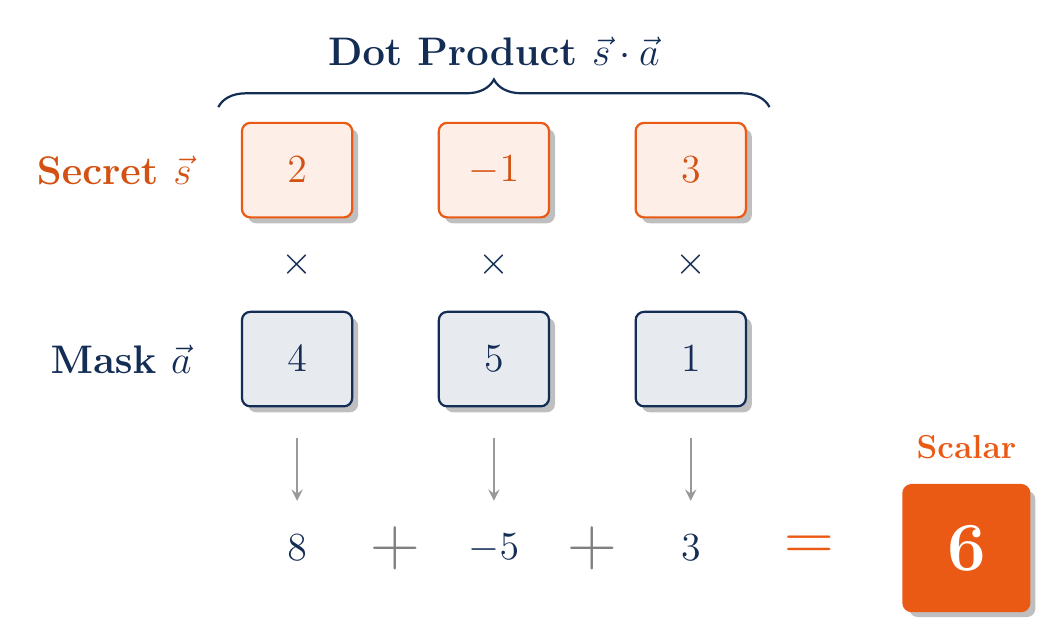
\begin{tikzpicture}[
            cell/.style={draw, thick, rounded corners=3pt, minimum width=1.4cm, minimum height=1.2cm, align=center, font=\Large\bfseries, drop shadow},
            secret/.style={cell, fill=AccentOrange!10, draw=AccentOrange, text=AccentOrange!90!black},
            mask/.style={cell, fill=DeepBlue!10, draw=DeepBlue, text=DeepBlue},
            math/.style={font=\Large\bfseries, DeepBlue},
            arrow/.style={->, thick, gray!80, >=stealth}
        ]
        
        % Vector S (Secret)
        \node[secret] (s1) at (0, 0) {$2$};
        \node[secret] (s2) at (2.5, 0) {$-1$};
        \node[secret] (s3) at (5.0, 0) {$3$};
        \node[left=0.5cm of s1, font=\Large\bfseries, AccentOrange!90!black] {Secret $\vec{s}$};
        
        % Multiplication symbols between vectors
        \node[math] at (0, -1.2) {$\times$};
        \node[math] at (2.5, -1.2) {$\times$};
        \node[math] at (5.0, -1.2) {$\times$};
        
        % Vector A (Mask)
        \node[mask] (a1) at (0, -2.4) {$4$};
        \node[mask] (a2) at (2.5, -2.4) {$5$};
        \node[mask] (a3) at (5.0, -2.4) {$1$};
        \node[left=0.5cm of a1, font=\Large\bfseries, DeepBlue] {Mask $\vec{a}$};
        
        % Arrows pointing down to the calculation
        \draw[arrow] (0, -3.4) -- (0, -4.2);
        \draw[arrow] (2.5, -3.4) -- (2.5, -4.2);
        \draw[arrow] (5.0, -3.4) -- (5.0, -4.2);
        
        % Step 3: Products and Addition
        \node[math] (m1) at (0, -4.8) {$8$};
        \node[math, text=gray] (p1) at (1.25, -4.8) {\Huge $+$};
        \node[math] (m2) at (2.5, -4.8) {$-5$};
        \node[math, text=gray] (p2) at (3.75, -4.8) {\Huge $+$};
        \node[math] (m3) at (5.0, -4.8) {$3$};
        
        % Final Scalar Result
        \node[math, text=AccentOrange] (eq) at (6.5, -4.8) {\Huge $=$};
        \node[cell, fill=AccentOrange, draw=AccentOrange, text=white, minimum width=1.6cm, minimum height=1.6cm] (res) at (8.5, -4.8) {\Huge 6};
        \node[above=0.2cm of res, font=\large\bfseries, AccentOrange] {Scalar};
        
        % Top Brace grouping the vectors
        \draw[thick, DeepBlue, decorate, decoration={brace, amplitude=10pt}] (-1, 0.8) -- (6.0, 0.8) node[midway, above=0.4cm, font=\Large\bfseries] {Dot Product $\vec{s} \cdot \vec{a}$};

        \end{tikzpicture}
    }
    \end{center}
\end{frame}


% ========================================== 
% SECTION 3
% ========================================== 
\section{The LWE Problem}

% --- SLAJD 1: Zwykłe układy równań (Łatwy problem) ---
\begin{frame}{The Foundation: Standard Linear Equations}
    \Large
    \textbf{Solving standard equations is easy.} \\
    \vspace{0.4cm}
    \normalsize
    Given enough equations, finding the exact secret values ($s_1, s_2$) is a trivial task for any modern computer (e.g., using Gaussian elimination).
    \vspace{0.4cm}

    \begin{block}{\faCheckCircle \ Standard Linear Equations}
        \centering
        \vspace{0.3cm}
        \Large $14 = 4s_1 + 3s_2$ \\
        \vspace{0.2cm}
        \Large $9 = 2s_1 + 1s_2$ \\
        \vspace{0.4cm}
        \Large \textbf{\textcolor{DeepBlue}{$\rightarrow s_1 = 3, s_2 = 2$}}
        \vspace{0.3cm}
    \end{block}
\end{frame}

% --- SLAJD 2: Wprowadzenie szumu (Problem LWE) ---
\begin{frame}{The Hard Problem: Learning With Errors (LWE)}
    \Large
    \textbf{What happens if we add a little noise?} \\
    \vspace{0.2cm}
    \normalsize
    If we intentionally add a tiny, random \textbf{error (noise)} to the end of each equation, the math completely "breaks".
    \vspace{0.2cm}

    \begin{alertblock}{\faLock \ Learning With Errors (LWE)}
        \centering
        \vspace{0.1cm}
        \Large 
        $15 = 4s_1 + 3s_2 + \textcolor{AccentOrange}{{e_1}}$ \\[0.2cm]
        $8 = 2s_1 + 1s_2 + \textcolor{AccentOrange}{{e_2}}$ \\[0.3cm]
        \textbf{\textcolor{AccentOrange}{$\rightarrow s_1 = \text{?}, s_2 = \text{?}$}}
        \vspace{0.1cm}
    \end{alertblock}
    \vspace{0.3cm}
    \centering
    \small \textit{Even quantum computers struggle to find $\vec{s}$ when noise is present!}
\end{frame}

\section{FHE Encryption}
% --- SLAJD 1: Krok 1 - Składniki (Wersja Uproszczona) ---
\begin{frame}{LWE Encryption: Step 1 - The Ingredients}
    \Large
    \textbf{How do we actually encrypt a number?} \\
    \vspace{0.2cm}
    \normalsize
    Before doing any math, we must gather our four cryptographic components.
    \vspace{0.4cm}
    
    \begin{block}{\faList \ System Setup \& Ingredients}
        \begin{itemize}
            \item \textbf{Secret Key ($\vec{s}$):} The master key used to both encrypt and decrypt the message.
            \item \textbf{Public Mask ($\vec{a}$):} A new, random vector generated entirely fresh \textit{for every single encryption}.
            \item \textbf{Noise ($e$):} The crucial tiny error that makes the system of equations impossible to solve.
            \item \textbf{Scaling Factor ($\Delta$):} A multiplier that shifts our message to the left, protecting it from being damaged by the noise.
        \end{itemize}
    \end{block}
    \vspace{0.2cm}
    \begin{center}
        \textit{\textcolor{gray}{Note: The vectors $\vec{s}$ and $\vec{a}$ must be the exact same length!}}
    \end{center}
\end{frame}

% --- SLAJD 2: Krok 2 - Przygotowanie ładunku ---
\begin{frame}{LWE Encryption: Step 2 - Preparing the Payload}
    \Large
    \textbf{Formatting the Data Box} \\
    \vspace{0.2cm}
    \normalsize
    We do not encrypt the raw message $m$ directly. First, we must construct the "Payload" (the data box we visualized earlier) by scaling the message and injecting the noise.
    \vspace{0.3cm}
    
    \begin{exampleblock}{\faBox \ Payload Construction}
        \centering
        \vspace{0.2cm}
        \Large $\text{Payload} = \Delta m + \textcolor{AccentOrange}{{e}}$
        \vspace{0.2cm}
    \end{exampleblock}
    \vspace{0.4cm}
    
    \begin{itemize}
        \item \textbf{Multiply by $\Delta$:} Shifts the message $m$ to the upper, significant bits.
        \item \textbf{Add Noise $e$:} Fills the empty lower bits with random Gaussian noise to guarantee security against attacks.
    \end{itemize}
\end{frame}


% --- SLAJD 1: Metafora powodzi (Brak skalowania) ---
\begin{frame}{Intuition: Without Scaling Factor (Disaster)}
    \Large \textbf{Leaving the data on the floor} \\
    \vspace{0.1cm}
    \normalsize
    Imagine our cryptographic space as a room. The random noise ($e$) we must add is like \textbf{floodwater} creeping across the floor. If we leave our valuable message ($m$) directly on the floor without scaling, it mixes with the noise.

    \vspace{0.1cm}
    \begin{center}
    % Zmniejszono do 0.60, aby na pewno zmieściło się w pionie
    \resizebox{0.60\textwidth}{!}{
        \begin{tikzpicture}[
            % Zmniejszono font na \large i wysokość klocka, aby był bardziej zwarty
            box/.style={draw=DeepBlue, ultra thick, minimum width=2.4cm, minimum height=1.2cm, align=center, font=\large\bfseries, fill=DeepBlue!80, text=white},
            wave_line/.style={decorate, decoration={snake, amplitude=1.2mm, segment length=5mm}, draw=cyan!60!blue, thick}
        ]
        
        % Podłoga
        \draw[ultra thick, gray] (-4,0) -- (4,0);
        
        % Wiadomość na podłodze - tekst w dwóch liniach, żeby klocek był węższy!
        \node[box, label=above:\textcolor{red}{\Large \faTimes \ Corrupted}] (msg) at (0, 0.6) {Raw Message \\ ($m$)};
        
        % WODA Z EFEKTEM BIAŁYCH SZCZYTÓW (Większa przezroczystość - opacity 0.55)
        % Używamy mocniejszego niebieskiego na dole, żeby przy opacity=0.55 wciąż wyglądał jak woda
        \fill[bottom color=cyan!90!blue, top color=white, opacity=0.55] 
            (-4,0) -- (-4, 0.8) 
            decorate[decoration={snake, amplitude=1.2mm, segment length=5mm}] { -- (4, 0.8) } 
            -- (4,0) -- cycle;
            
        % Cienka linia fali na samej górze - przesunięto napis mocniej w prawo (pos=0.92)
        \draw[wave_line] (-4, 0.8) -- (4, 0.8) node[pos=0.92, above=0.05cm, text=cyan!80!blue, font=\bfseries] {Noise ($e$)};

        % Oś bitów (Z prawej strony) - Skrócona do 2.4, żeby uciąć zbędną wysokość obrazka
        \draw[->, thick, gray] (4.8, 0) -- (4.8, 2.4) node[above, font=\bfseries] {Bits};
        \node[right, font=\bfseries, text=cyan!80!blue] at (4.9, 0.4) {LSB (Floor)};

        \end{tikzpicture}
    }
    \end{center}
    \vspace{0.1cm}
    \centering
    \textit{\textcolor{gray}{\small $\rightarrow$ Result: The message and noise overlap in the LSB. Irreversible decryption failure!}}
\end{frame}

% --- SLAJD 2: Metafora powodzi (Zastosowanie skalowania) ---
\begin{frame}{Intuition: With Scaling Factor (Safe)}
    \Large \textbf{Building a high shelf ($\Delta$)} \\
    \vspace{0.1cm}
    \normalsize
    Multiplying $m$ by the scaling factor $\Delta$ is like \textbf{building a high shelf}. We safely lift the message to the top shelf, leaving the floodwater harmlessly on the floor.

    \vspace{0.1cm}
    \begin{center}
    % Skala 0.55 gwarantuje, że wyższy rysunek bez problemu zmieści się na slajdzie
    \resizebox{0.55\textwidth}{!}{
        \begin{tikzpicture}[
            box/.style={draw=DeepBlue, ultra thick, minimum width=2.4cm, minimum height=1.2cm, align=center, font=\large\bfseries, fill=DeepBlue!80, text=white},
            wave_line/.style={decorate, decoration={snake, amplitude=1.2mm, segment length=5mm}, draw=cyan!60!blue, thick}
        ]
        
        % Podłoga
        \draw[ultra thick, gray] (-4,0) -- (4,0);
        
        % Półka (Czynnik skalujący Delta) - od 0 do 1.5, żeby nie zajmować za dużo miejsca w pionie
        \draw[ultra thick, DeepBlue!70, fill=DeepBlue!10] (-1.2, 0) rectangle (1.2, 1.5);
        \node[font=\huge\bfseries, text=DeepBlue!50] at (0, 0.75) {$\times \Delta$};
        
        % Wiadomość bezpieczna na półce - tekst w dwóch liniach dla spójności i wąskiego klocka
        % Środek wiadomości jest na wysokości 2.1 (dolna krawędź idealnie na półce)
        \node[box, label=above:\textcolor{green!60!black}{\Large \faCheck \ Safe}] at (0, 2.1) {Scaled Msg \\ ($\Delta m$)};
        
        % WODA Z EFEKTEM BIAŁYCH SZCZYTÓW (Dokładnie taka sama jak na slajdzie 1)
        \fill[bottom color=cyan!90!blue, top color=white, opacity=0.55] 
            (-4,0) -- (-4, 0.8) 
            decorate[decoration={snake, amplitude=1.2mm, segment length=5mm}] { -- (4, 0.8) } 
            -- (4,0) -- cycle;
            
        % Cienka linia fali na samej górze - przesunięta w prawo
        \draw[wave_line] (-4, 0.8) -- (4, 0.8) node[pos=0.92, above=0.05cm, text=cyan!80!blue, font=\bfseries] {Noise ($e$)};

        % Oś bitów (Z prawej strony) - Sięga wyżej (3.2), żeby objąć półkę
        \draw[->, thick, gray] (4.8, 0) -- (4.8, 3.2) node[above, font=\bfseries] {Bits};
        \node[right, font=\bfseries, text=cyan!80!blue] at (4.9, 0.4) {LSB (Floor)};
        \node[right, font=\bfseries, text=DeepBlue] at (4.9, 2.1) {MSB (Shelf)};

        \end{tikzpicture}
    }
    \end{center}
    \vspace{0.1cm}
    \centering
    \large \textbf{The Payload:} \quad $\underbrace{\Delta m}_{\text{Top Shelf (MSB)}} + \underbrace{e}_{\text{Floodwater (LSB)}}$
\end{frame}


% --- SLIDE 1: Raw Message ---
\begin{frame}{Visualizing the "Data Box" (1/3)}
    \textbf{Step 1: Raw Message.} We start with the raw message ($m$) in the least significant bits (LSB).
    \vspace{0.6cm}
    
    {\centering
    \resizebox{0.75\textwidth}{!}{
        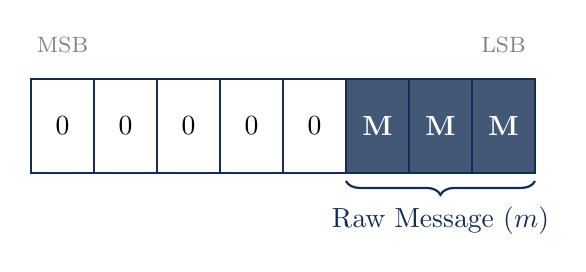
\begin{tikzpicture}[
            bit/.style={draw=DeepBlue, thick, minimum width=0.8cm, minimum height=1.2cm, fill=white},
            msg/.style={fill=DeepBlue!80, text=white, font=\bfseries}
        ]
        
        % The Box
        \node[bit] (b1) at (0,0) {0};
        \node[bit] (b2) at (0.8,0) {0};
        \node[bit] (b3) at (1.6,0) {0};
        \node[bit] (b4) at (2.4,0) {0};
        \node[bit] (b5) at (3.2,0) {0};
        \node[bit, msg] (b6) at (4.0,0) {M};
        \node[bit, msg] (b7) at (4.8,0) {M};
        \node[bit, msg] (b8) at (5.6,0) {M};
        
        % Labels
        \draw[thick, DeepBlue, decorate, decoration={brace, amplitude=5pt, mirror}] (3.6, -0.7) -- (6.0, -0.7) node[midway, below=0.2cm] {Raw Message ($m$)};
        
        \node[above=0.2cm of b1, font=\footnotesize, text=gray] {MSB};
        \node[above=0.2cm of b8, font=\footnotesize, text=gray] {LSB};

        \end{tikzpicture}
    }\par}
    \vspace{0.4cm}
\end{frame}

% --- SLIDE 2: Scaled Message ---
\begin{frame}{Visualizing the "Data Box" (2/3)}
    \textbf{Step 2: Scaling.} Multiplying by $\Delta$ shifts the message to the most significant bits (MSB).
    \vspace{0.6cm}
    
    {\centering
    \resizebox{0.75\textwidth}{!}{
        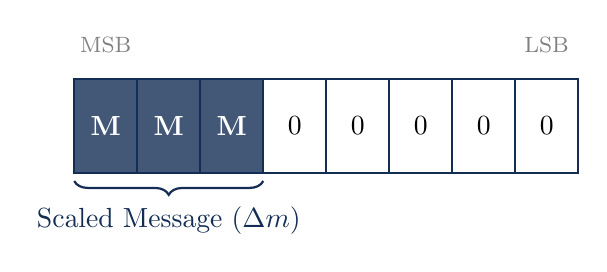
\begin{tikzpicture}[
            bit/.style={draw=DeepBlue, thick, minimum width=0.8cm, minimum height=1.2cm, fill=white},
            msg/.style={fill=DeepBlue!80, text=white, font=\bfseries}
        ]
        
        % The Box
        \node[bit, msg] (b1) at (0,0) {M};
        \node[bit, msg] (b2) at (0.8,0) {M};
        \node[bit, msg] (b3) at (1.6,0) {M};
        \node[bit] (b4) at (2.4,0) {0};
        \node[bit] (b5) at (3.2,0) {0};
        \node[bit] (b6) at (4.0,0) {0};
        \node[bit] (b7) at (4.8,0) {0};
        \node[bit] (b8) at (5.6,0) {0};
        
        % Labels
        \draw[thick, DeepBlue, decorate, decoration={brace, amplitude=5pt, mirror}] (-0.4, -0.7) -- (2.0, -0.7) node[midway, below=0.2cm] {Scaled Message ($\Delta m$)};
        
        \node[above=0.2cm of b1, font=\footnotesize, text=gray] {MSB};
        \node[above=0.2cm of b8, font=\footnotesize, text=gray] {LSB};

        \end{tikzpicture}
    }\par}
    \vspace{0.4cm}
\end{frame}

% --- SLIDE 3: Adding Noise ---
\begin{frame}{Visualizing the "Data Box" (3/3)}
    \textbf{Step 3: Adding Noise.} We safely hide the random noise ($e$) in the empty lower bits.
    \vspace{0.6cm}
    
    {\centering
    \resizebox{0.75\textwidth}{!}{
        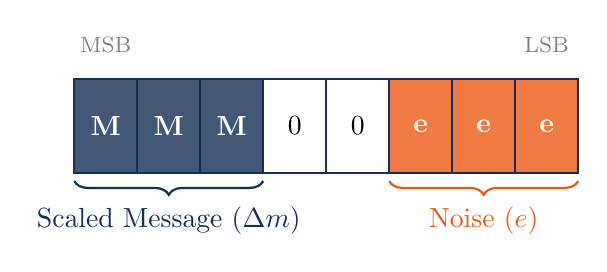
\begin{tikzpicture}[
            bit/.style={draw=DeepBlue, thick, minimum width=0.8cm, minimum height=1.2cm, fill=white},
            msg/.style={fill=DeepBlue!80, text=white, font=\bfseries},
            noise/.style={fill=AccentOrange!80, text=white, font=\bfseries}
        ]
        
        % The Box
        \node[bit, msg] (b1) at (0,0) {M};
        \node[bit, msg] (b2) at (0.8,0) {M};
        \node[bit, msg] (b3) at (1.6,0) {M};
        \node[bit] (b4) at (2.4,0) {0};
        \node[bit] (b5) at (3.2,0) {0};
        \node[bit, noise] (b6) at (4.0,0) {e};
        \node[bit, noise] (b7) at (4.8,0) {e};
        \node[bit, noise] (b8) at (5.6,0) {e};
        
        % Labels
        \draw[thick, DeepBlue, decorate, decoration={brace, amplitude=5pt, mirror}] (-0.4, -0.7) -- (2.0, -0.7) node[midway, below=0.2cm] {Scaled Message ($\Delta m$)};
        \draw[thick, AccentOrange, decorate, decoration={brace, amplitude=5pt, mirror}] (3.6, -0.7) -- (6.0, -0.7) node[midway, below=0.2cm] {Noise ($e$)};
        
        \node[above=0.2cm of b1, font=\footnotesize, text=gray] {MSB};
        \node[above=0.2cm of b8, font=\footnotesize, text=gray] {LSB};

        \end{tikzpicture}
    }\par}
    \vspace{0.4cm}
\end{frame}

% --- SLAJD 1: LWE - Faza 1: Składniki (Z uproszczonym Payloadem) ---
\begin{frame}{LWE Encryption: Phase 1 - The Ingredients}
    \Large \textbf{Gathering the Components} \\
    \vspace{0.2cm}
    \normalsize
    Since we already prepared our \textbf{Payload} ($\Delta m + e$) in the previous step, we now only need three main components on the table:
    \vspace{0.8cm}
    
    \begin{columns}[T]
        % Kolumna 1: Maska
        \begin{column}{0.33\textwidth}
            \centering
            \textcolor{AccentOrange}{\Huge \faDice} \\ \vspace{0.3cm}
            \textbf{New Mask ($\vec{a}$)} \\
            \vspace{0.1cm}
            \small A completely fresh, random public vector.
        \end{column}
        
        % Kolumna 2: Klucz
        \begin{column}{0.33\textwidth}
            \centering
            \textcolor{DeepBlue}{\Huge \faKey} \\ \vspace{0.3cm}
            \textbf{Secret Key ($\vec{s}$)} \\
            \vspace{0.1cm}
            \small Our static master key.
        \end{column}
        
        % Kolumna 3: Payload
        \begin{column}{0.33\textwidth}
            \centering
            \textcolor{DeepBlue}{\Huge \faBox} \\ \vspace{0.3cm}
            \textbf{Prepared Payload} \\
            \vspace{0.1cm}
            \small The data box ($\Delta m + e$) we just built.
        \end{column}
    \end{columns}
\end{frame}

% --- SLAJD 2: LWE - Faza 2: Obliczenia ---
\begin{frame}{LWE Encryption: Phase 2 - The Calculation}
    \Large \textbf{Locking the Payload} \\
    \vspace{0.1cm}
    \normalsize
    Now we mathematically add the prepared \textbf{Payload} to our cryptographic lock (the dot product) to completely scramble the data:
    \vspace{0.3cm}
    
    \begin{alertblock}{\faCalculator \ The Encryption Equation}
        \centering
        \vspace{0.2cm}
        \Large $b = \underbrace{(\vec{a} \cdot \vec{s})}_{\text{Lock}} + \underbrace{\text{Payload}}_{\Delta m + e} \pmod q$
        \vspace{0.2cm}
    \end{alertblock}
    \vspace{0.4cm}
    
    \begin{center}
        % Złączenie tekstu i wzoru w jednej linii za pomocą \quad (odstęp poziomy)
        \large \textbf{The Final Ciphertext Pair:} \quad \Large ${CT = (\vec{a}, b)}$
    \end{center}
\end{frame}


% --- SLAJD 2: LWE - Wizualizacja przepływu (Zaktualizowana) ---
\begin{frame}{LWE Encryption: Visualizing the Flow}
    \vspace{0.2cm}
    {\centering
    \resizebox{0.95\textwidth}{!}{
        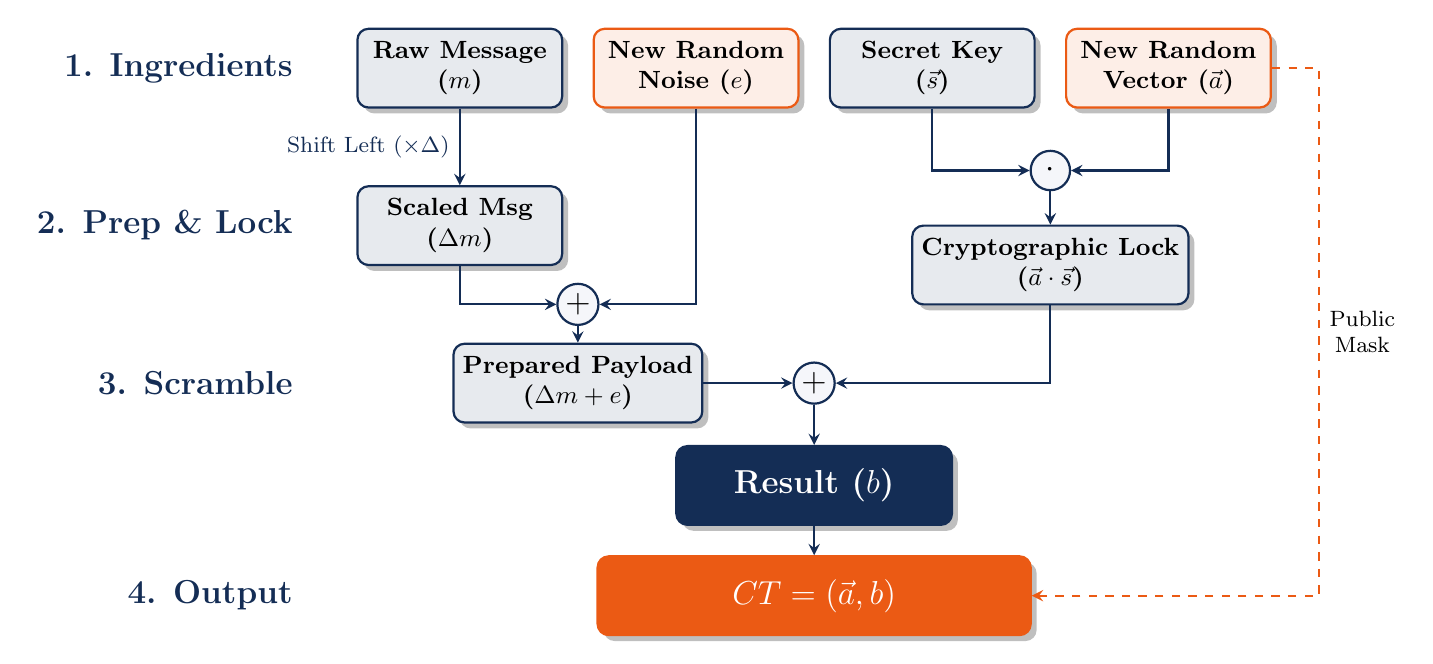
\begin{tikzpicture}[
            >=stealth,
            box/.style={draw=DeepBlue, thick, fill=white, rounded corners, minimum width=2.6cm, minimum height=1.0cm, align=center, font=\small\bfseries, drop shadow},
            fresh/.style={box, fill=AccentOrange!10, draw=AccentOrange}, % Nowe/Losowe
            static/.style={box, fill=DeepBlue!10}, % Stałe
            op/.style={draw=DeepBlue, thick, circle, fill=LightGray, minimum size=0.5cm, font=\large\bfseries, inner sep=1pt},
            result/.style={draw=DeepBlue, thick, fill=DeepBlue, text=white, rounded corners, minimum width=3.5cm, minimum height=1.0cm, align=center, font=\large\bfseries, drop shadow}
        ]

        % --- ETYKIETY FAZ (Z LEWEJ STRONY) ---
        \node[font=\large\bfseries, DeepBlue, anchor=east] at (-6.5, 4.5) {1. Ingredients};
        \node[font=\large\bfseries, DeepBlue, anchor=east] at (-6.5, 2.5) {2. Prep \& Lock};
        \node[font=\large\bfseries, DeepBlue, anchor=east] at (-6.5, 0.5) {3. Scramble};
        \node[font=\large\bfseries, DeepBlue, anchor=east] at (-6.5, -2.2) {4. Output};

        % --- POZIOM 1: Składniki ---
        \node[static] (msg) at (-4.5, 4.5) {Raw Message \\ ($m$)};
        \node[fresh] (noise) at (-1.5, 4.5) {New Random \\ Noise ($e$)};
        \node[static] (key) at (1.5, 4.5) {Secret Key \\ ($\vec{s}$)};
        \node[fresh] (mask) at (4.5, 4.5) {New Random \\ Vector ($\vec{a}$)};

        % --- POZIOM 2: Przygotowanie Payloadu (Lewa) i Kłódki (Prawa) ---
        % Lewa strona: Payload
        \node[static] (scaled) at (-4.5, 2.5) {Scaled Msg \\ ($\Delta m$)};
        \draw[->, thick, DeepBlue] (msg) -- (scaled) node[midway, left, font=\footnotesize] {Shift Left ($\times \Delta$)};

        \node[op] (plus_payload) at (-3.0, 1.5) {$+$};
        \draw[->, thick, DeepBlue] (scaled) |- (plus_payload);
        \draw[->, thick, DeepBlue] (noise) |- (plus_payload);

        \node[static, minimum width=2.8cm] (payload) at (-3.0, 0.5) {Prepared Payload \\ ($\Delta m + e$)};
        \draw[->, thick, DeepBlue] (plus_payload) -- (payload);

        % Prawa strona: Kłódka (Lock)
        \node[op] (dot_lock) at (3.0, 3.2) {$\cdot$};
        \draw[->, thick, DeepBlue] (key) |- (dot_lock);
        \draw[->, thick, DeepBlue] (mask) |- (dot_lock);

        \node[static, minimum width=2.8cm] (lock) at (3.0, 2.0) {Cryptographic Lock \\ ($\vec{a} \cdot \vec{s}$)};
        \draw[->, thick, DeepBlue] (dot_lock) -- (lock);

        % --- POZIOM 3: Łączenie (Scramble) ---
        \node[op] (plus_b) at (0, 0.5) {$+$};
        \draw[->, thick, DeepBlue] (payload) -- (plus_b);
        \draw[->, thick, DeepBlue] (lock) |- (plus_b);

        \node[result] (b) at (0, -0.8) {Result ($b$)};
        \draw[->, thick, DeepBlue] (plus_b) -- (b);

        % --- POZIOM 4: Wynik Końcowy ---
        \node[result, minimum width=5.5cm, fill=AccentOrange, draw=AccentOrange] (ct) at (0, -2.2) {${CT = (\vec{a}, b)}$};
        \draw[->, thick, DeepBlue] (b) -- (ct);

        % Linia dla maski (Omijająca cały diagram z prawej strony)
        \draw[->, thick, AccentOrange, dashed] (mask.east) -- ++(0.6, 0) coordinate (A) -- (A |- ct.east) node[midway, right, font=\footnotesize, text=black, align=center] {Public\\Mask} -- (ct.east);

        \end{tikzpicture}
    }\par}
\end{frame}





% --- SLAJD 4: Deszyfrowanie LWE (Krok 1) ---
\section{LWE Decryption}
\begin{frame}{LWE Decryption: Step 1 - Removing the Mask}
    \Large
    \textbf{How do we get our message back?} \\
    \vspace{0.2cm}
    \normalsize
    To decrypt the ciphertext ${CT = (\vec{a}, b)}$, the receiver uses their Secret Key ($\vec{s}$) to reverse the encryption. The first step is to remove the cryptographic lock.
    \vspace{0.4cm}
    
    \begin{block}{\faUnlock \ Step 1: Remove the Mask}
        \centering
        \vspace{0.2cm}
        \Large $b - (\vec{a} \cdot \vec{s}) = \Delta m + \textcolor{AccentOrange}{{e}}$
        \vspace{0.2cm}
    \end{block}
    \vspace{0.4cm}
    
    \begin{center}
        \textit{\textcolor{gray}{By mathematically subtracting the mask ($\vec{a} \cdot \vec{s}$), we successfully unlock the ciphertext. We are now left with the "Data Box" containing our scaled message and the noise.}}
    \end{center}
\end{frame}

% --- SLAJD 5: Deszyfrowanie LWE (Krok 2) ---
\begin{frame}{LWE Decryption: Step 2 - Extracting the Message}
    \Large
    \textbf{Destroying the Noise} \\
    \vspace{0.2cm}
    \normalsize
    Now that we have the exposed payload ($\Delta m + e$), we need to extract the raw message $m$ without the noise.
    \vspace{0.4cm}
    
    \begin{exampleblock}{\faCheckCircle \ Step 2: Scale Down and Round}
        \centering
        \vspace{0.2cm}
        \Large $\left\lfloor \frac{\Delta m + \textcolor{AccentOrange}{{e}}}{\Delta} \right\rceil = m$
        \vspace{0.2cm}
    \end{exampleblock}
    \vspace{0.4cm}
    
    \begin{center}
        \textbf{The Magic of Rounding:} \\
        Dividing by $\Delta$ and rounding to the nearest integer completely destroys the noise $e$, restoring the perfect message $m$! \\
        \vspace{0.3cm}
        \textit{\textcolor{gray}{\small (This works flawlessly, provided the noise is small enough: $e < \Delta / 2$)}}
    \end{center}
\end{frame}

% --- SLAJD: LWE Decryption - Wizualizacja przepływu (Finalna wersja) ---
\begin{frame}{LWE Decryption: Visualizing the Flow}
    \vspace{0.1cm}
    {\centering
    \resizebox{0.86\textwidth}{!}{
        \begin{tikzpicture}[
            >=stealth,
            box/.style={draw=DeepBlue, thick, fill=white, rounded corners, minimum width=2.6cm, minimum height=0.7cm, align=center, font=\small\bfseries, drop shadow},
            fresh/.style={box, fill=AccentOrange!10, draw=AccentOrange}, % Szyfrogram
            static/.style={box, fill=DeepBlue!10}, % Klucz i Payload
            op/.style={draw=DeepBlue, thick, circle, fill=LightGray, minimum size=0.4cm, font=\large\bfseries, inner sep=1pt},
            result/.style={draw=green!60!black, thick, fill=green!60!black, text=white, rounded corners, minimum width=3.2cm, minimum height=0.7cm, align=center, font=\large\bfseries, drop shadow}
        ]

        % --- POZIOM 1: Wejścia ---
        \node[static] (key) at (-6.0, 3.0) {Secret Key \\ ($\vec{s}$)};
        \node[fresh] (mask) at (-1.5, 3.0) {Public Mask \\ ($\vec{a}$)};
        \node[fresh] (b) at (5.5, 3.0) {Scrambled Value \\ ($b$)};

        % KLAMRA (Obejmuje tylko wektory a oraz b)
        \draw[thick, AccentOrange, decorate, decoration={brace, amplitude=5pt}] 
            ([yshift=0.2cm]mask.north west) -- ([yshift=0.2cm]b.north east) 
            node[midway, above=0.2cm, font=\bfseries] {Received Ciphertext Pair ${CT = (\vec{a}, b)}$};

        % --- POZIOM 2: Odtworzenie kłódki ---
        \node[op] (dot) at (-3.75, 2.0) {$\cdot$};
        \draw[->, thick, DeepBlue] (key) |- (dot);
        \draw[->, thick, DeepBlue] (mask) |- (dot);

        \node[static, minimum width=2.8cm] (lock) at (-3.75, 1.2) {Reconstructed Lock \\ ($\vec{a} \cdot \vec{s}$)};
        \draw[->, thick, DeepBlue] (dot) -- (lock);

        % --- POZIOM 2b: Odejmowanie ---
        \node[op] (minus) at (1.5, 0.4) {$-$};
        \draw[->, thick, DeepBlue] (lock) |- (minus);
        \draw[->, thick, DeepBlue] (b) |- (minus);

        % --- POZIOM 3: Payload i Zaokrąglanie (ZWIĘKSZONE ODSTĘPY) ---
        \node[static, minimum width=2.8cm] (payload) at (1.5, -0.6) {Recovered Payload \\ ($\Delta m + e$)};
        \draw[->, thick, DeepBlue] (minus) -- (payload);

        \node[box, fill=LightGray, minimum width=3.0cm] (round) at (1.5, -2.0) {Scale Down \& Round \\ $\lfloor \frac{\Delta m + e}{\Delta} \rceil$};
        \draw[->, thick, DeepBlue] (payload) -- (round);

        % Etykieta usuwania szumu
        \node[right=0.2cm of round, font=\small\bfseries, text=AccentOrange, align=left] {\faTrash \ Noise ($e$) \\ is destroyed!};

        % --- POZIOM 4: Wynik Końcowy ---
        \node[result] (msg) at (1.5, -3.4) {\faUnlock \ Original Message ($m$)};
        \draw[->, thick, DeepBlue] (round) -- (msg);

        % --- ETYKIETY FAZ (Z LEWEJ STRONY) ---
        \node[font=\large\bfseries, DeepBlue, anchor=east] at (-8.5, 3.0) {1. Inputs};
        \node[font=\large\bfseries, DeepBlue, anchor=east] at (-8.5, 1.2) {2. Remove Mask};
        \node[font=\large\bfseries, DeepBlue, anchor=east] at (-8.5, -1.3) {3. Destroy Noise};
        \node[font=\large\bfseries, DeepBlue, anchor=east] at (-8.5, -3.4) {4. Output};

        \end{tikzpicture}
    }\par}
\end{frame}

% ========================================== 
% SECTION 4
% ========================================== 

% --- SLAJD 1: Dodawanie Homomorficzne - Szyfrowanie ---
\section{Homomorphic Addition}
\begin{frame}{Homomorphic Addition: Step 1 - Two Messages}
    \Large
    \textbf{Setting up the scenario} \\
    \vspace{0.2cm}
    \normalsize
    Let's encrypt two different messages, $m_1$ and $m_2$, using the exact same Secret Key ($\vec{s}$). Notice that each gets a completely new mask and new noise!
    \vspace{0.3cm}
    
    \begin{block}{\faLock \ Ciphertext 1}
        \centering
        \large ${CT_1} = (\vec{a}_1, \ b_1)$ \quad \textit{where} \quad $b_1 = (\vec{a}_1 \cdot \vec{s}) + \Delta m_1 + \textcolor{AccentOrange}{{e_1}}$
        \vspace{0.1cm}
    \end{block}
    \vspace{0.2cm}
    
    \begin{block}{\faLock \ Ciphertext 2}
        \centering
        \large ${CT_2} = (\vec{a}_2, \ b_2)$ \quad \textit{where} \quad $b_2 = (\vec{a}_2 \cdot \vec{s}) + \Delta m_2 + \textcolor{AccentOrange}{{e_2}}$
        \vspace{0.1cm}
    \end{block}
\end{frame}

% --- SLAJD 2: Dodawanie Homomorficzne - Chmura ---
\begin{frame}{Homomorphic Addition: Step 2 - Cloud Computation}
    \Large
    \textbf{Adding blindly in the cloud} \\
    \vspace{0.2cm}
    \normalsize
    The server does not know $\vec{s}$, $m_1$, or $m_2$. It simply adds the public vectors and the scalars together.
    \vspace{0.3cm}
    
    \begin{exampleblock}{\faCloud \ Computing $CT_{SUM}$}
        \centering
        \vspace{0.2cm}
        \Large ${CT_{SUM}} = (\vec{a}_1 + \vec{a}_2, \ b_1 + b_2)$
        \vspace{0.2cm}
    \end{exampleblock}
    \vspace{0.3cm}
    
    \textbf{What happened inside the new scalar?} \\
    If we mathematically expand $b_1 + b_2$, the math perfectly aligns:
    \[ b_{SUM} = (\vec{a}_1 + \vec{a}_2) \cdot \vec{s} + \Delta(m_1 + m_2) + \textcolor{AccentOrange}{{(e_1 + e_2)}} \]
\end{frame}

% --- SLAJD 3: Dodawanie Homomorficzne - Deszyfrowanie ---
\begin{frame}{Homomorphic Addition: Step 3 - The Magic of Decryption}
    \Large
    \textbf{Unlocking the sum} \\
    \vspace{0.2cm}
    \normalsize
    The receiver downloads $CT_{SUM}$ and uses their Secret Key ($\vec{s}$) to decrypt it exactly like a normal ciphertext!
    \vspace{0.2cm}
    
    \begin{alertblock}{\faUnlock \ 1. Remove the combined mask}
        \centering
        \vspace{0.15cm}
        \large $b_{SUM} - (\vec{a}_1 + \vec{a}_2) \cdot \vec{s} = \Delta(m_1 + m_2) + \textcolor{AccentOrange}{{(e_1 + e_2)}}$
        \vspace{0.15cm}
    \end{alertblock}
    \vspace{0.2cm}
    
    \begin{exampleblock}{\faCheckCircle \ 2. Scale down and round}
        \centering
        \vspace{0.15cm}
        \large $\left\lfloor \frac{\Delta(m_1 + m_2) + \textcolor{AccentOrange}{{(e_1 + e_2)}}}{\Delta} \right\rceil = {m_1 + m_2}$
        \vspace{0.15cm}
    \end{exampleblock}
    \vspace{0.1cm}
    \centering
    \textit{\textcolor{gray}{\small The messages added up cleanly, and the noises just gently added together!}}
\end{frame}

% --- SLAJD: Metafora powodzi (Dodawanie Homomorficzne) ---
\begin{frame}{Intuition: Homomorphic Addition (Safe)}
    \Large \textbf{The floodwater rises, but the shelf is high} \\
    \vspace{0.1cm}
    \normalsize
    When we homomorphically add two ciphertexts, the messages add up safely on the top shelf ($m_1 + m_2$). The random noises also add up ($e_1 + e_2$), causing the floodwater to rise. However, it is still far from reaching the data!

    \vspace{0.1cm}
    \begin{center}
    % Zmniejszona skala (z 0.58 na 0.53), aby slajd miał więcej oddechu w pionie
    \resizebox{0.53\textwidth}{!}{
        \begin{tikzpicture}[
            box/.style={draw=DeepBlue, ultra thick, minimum width=2.6cm, minimum height=1.2cm, align=center, font=\large\bfseries, fill=DeepBlue!80, text=white},
            wave_line/.style={decorate, decoration={snake, amplitude=1.2mm, segment length=5mm}, draw=cyan!60!blue, thick}
        ]
        
        % Podłoga
        \draw[ultra thick, gray] (-4,0) -- (4,0);
        
        % Półka (Czynnik skalujący Delta)
        \draw[ultra thick, DeepBlue!70, fill=DeepBlue!10] (-1.3, 0) rectangle (1.3, 1.8);
        \node[font=\huge\bfseries, text=DeepBlue!50] at (0, 0.9) {$\times \Delta$};
        
        % Wiadomość bezpieczna na półce
        \node[box, label=above:\textcolor{green!60!black}{\Large \faCheck \ Safe}] at (0, 2.4) {Summed Msg \\ ($m_1 + m_2$)};
        
        % WODA Z EFEKTEM BIAŁYCH SZCZYTÓW - Poziom wody ZNACZNIE WYŻSZY (y=1.2)
        \fill[bottom color=cyan!90!blue, top color=white, opacity=0.55] 
            (-4,0) -- (-4, 1.2) 
            decorate[decoration={snake, amplitude=1.2mm, segment length=5mm}] { -- (4, 1.2) } 
            -- (4,0) -- cycle;
            
        % Cienka linia fali na samej górze
        \draw[wave_line] (-4, 1.2) -- (4, 1.2) node[pos=0.88, above=0.05cm, text=cyan!80!blue, font=\bfseries, align=center] {Combined Noise \\ ($e_1 + e_2$)};

        % Oś bitów (Z prawej strony)
        \draw[->, thick, gray] (4.8, 0) -- (4.8, 3.6) node[above, font=\bfseries] {Bits};
        \node[right, font=\bfseries, text=cyan!80!blue] at (4.9, 0.6) {LSB (Floor)};
        \node[right, font=\bfseries, text=DeepBlue] at (4.9, 2.4) {MSB (Shelf)};

        \end{tikzpicture}
    }
    \end{center}
    \vspace{0.1cm}
    \centering
    \large \textbf{The Payload:} \quad $\underbrace{\Delta(m_1 + m_2)}_{\text{Top Shelf (MSB)}} + \underbrace{(e_1 + e_2)}_{\text{Floodwater (LSB)}}$
\end{frame}

% --- SLAJD: Turing Completeness ---
\begin{frame}{The Missing Piece: Turing Completeness}
    \Large \textbf{Why do we need both operations?} \\
    \vspace{0.1cm}
    \normalsize
    Partial homomorphism is not enough. To run arbitrary software or evaluate AI models, our system must be \textbf{Turing Complete}. In binary logic, every possible program can be built using just two basic operations:

    \vspace{0.1cm}
    \begin{center}
    \resizebox{0.7\textwidth}{!}{
        \begin{tikzpicture}[
            gate/.style={draw, ultra thick, minimum width=3cm, minimum height=1.2cm, align=center, font=\large\bfseries, fill=white, rounded corners},
            program/.style={draw=DeepBlue, ultra thick, minimum width=3.5cm, minimum height=2.5cm, align=center, font=\Large\bfseries, fill=DeepBlue!10, rounded corners, drop shadow},
            arrow/.style={->, ultra thick, gray, >=stealth}
        ]

        % Bramki logiczne
        \node[gate, draw=DeepBlue, text=DeepBlue] (xor) at (0, 1.5) {XOR Gate \\ \normalsize $a + b \pmod 2$};
        \node[gate, draw=AccentOrange, text=AccentOrange] (and) at (0, -1.5) {AND Gate \\ \normalsize $a \cdot b \pmod 2$};

        % Etykiety z operacjami FHE
        \node[left=0.5cm of xor, text=DeepBlue, font=\bfseries, align=right] {Homomorphic \\ \textbf{Addition}};
        \node[left=0.5cm of and, text=AccentOrange, font=\bfseries, align=right] {Homomorphic \\ \textbf{Multiplication}};

        % Znak Plusa (łączenie bramek)
        \node[font=\Huge\bfseries, text=gray] at (3.5, 0) {$+$};

        % Linie łączące bramki ze znakiem plusa
        \draw[ultra thick, gray] (xor.east) -| (3.5, 0.5);
        \draw[ultra thick, gray] (and.east) -| (3.5, -0.5);

        % Komputer w chmurze (Turing Complete)
        \node[program] (turing) at (7.5, 0) {\faCloud \ Cloud AI \\ \vspace{0.1cm} \normalsize (Turing Complete)};

        % Finałowa strzałka
        \draw[arrow] (4.0, 0) -- (turing.west);

        \end{tikzpicture}
    }
    \end{center}
    \vspace{0.2cm}
    \centering
    \textit{\textcolor{gray}{\small $\rightarrow$ We successfully conquered addition. Now, we must face the ultimate challenge: Multiplication!}}
\end{frame}


% --- SLAJD 1: Mnożenie Homomorficzne - Szyfrowanie ---
\section{Homomorphic Multiplication}
\begin{frame}{Homomorphic Multiplication: Step 1 - Two Messages}
    \Large
    \textbf{Setting up the scenario} \\
    \vspace{0.2cm}
    \normalsize
    Just like with addition, we start with two completely different messages, $m_1$ and $m_2$, encrypted under the same Secret Key ($\vec{s}$).
    \vspace{0.3cm}
    
    \begin{block}{\faLock \ Ciphertext 1}
        \centering
        \large ${CT_1} = (\vec{a}_1, \ b_1)$ \quad \textit{where} \quad $b_1 = (\vec{a}_1 \cdot \vec{s}) + \Delta m_1 + \textcolor{AccentOrange}{{e_1}}$
        \vspace{0.1cm}
    \end{block}
    \vspace{0.2cm}
    
    \begin{block}{\faLock \ Ciphertext 2}
        \centering
        \large ${CT_2} = (\vec{a}_2, \ b_2)$ \quad \textit{where} \quad $b_2 = (\vec{a}_2 \cdot \vec{s}) + \Delta m_2 + \textcolor{AccentOrange}{{e_2}}$
        \vspace{0.1cm}
    \end{block}
\end{frame}

% --- SLAJD 2a: Mnożenie Homomorficzne - Chmura (Równanie) ---
\begin{frame}{Homomorphic Multiplication: Step 2 - Cloud Computation}
    \Large
    \textbf{Multiplying in the cloud} \\
    \vspace{0.2cm}
    \normalsize
    The server multiplies the ciphertexts. Unlike simple addition, this requires complex mathematical operations, but let's focus purely on what happens inside the "Data Box" (the payload).
    \vspace{0.4cm}
    
    \begin{alertblock}{\faTimes \ Multiplying the Payloads}
        \centering
        \vspace{0.4cm}
        \large $(\Delta m_1 + e_1) \cdot (\Delta m_2 + e_2)$ \\[0.5cm]
        \Large $= \Delta^2(m_1 \cdot m_2) + \textcolor{AccentOrange}{\underbrace{\Delta(m_1 e_2 + m_2 e_1) + e_1 e_2}_{{E_{mult}}}}$
        \vspace{0.4cm}
    \end{alertblock}
\end{frame}

% --- SLAJD: Metafora powodzi (Mnożenie Homomorficzne) ---
\begin{frame}{Intuition: Homomorphic Multiplication (Danger)}
    \Large \textbf{The "Noise Explosion" tsunami} \\
    \vspace{0.1cm}
    \normalsize
    When we multiply ciphertexts, the cross-terms multiply the noise by the massive scaling factor $\Delta$. The floodwater rapidly surges into a \textbf{tsunami}. It is much higher than in addition and almost reaches the data! It is \textbf{barely safe} now, but \textbf{one more multiplication} will definitely cause an overflow and irreversibly destroy the message.

    \vspace{0.1cm}
    \begin{center}
    % Zmniejszono z 0.53 na 0.47 dla idealnego dopasowania w pionie
    \resizebox{0.44\textwidth}{!}{
        \begin{tikzpicture}[
            box/.style={draw=DeepBlue, ultra thick, minimum width=2.6cm, minimum height=1.2cm, align=center, font=\large\bfseries, fill=DeepBlue!80, text=white},
            wave_line/.style={decorate, decoration={snake, amplitude=1.2mm, segment length=5mm}, draw=cyan!60!blue, thick}
        ]
        
        % Podłoga
        \draw[ultra thick, gray] (-4,0) -- (4,0);
        
        % Półka (Czynnik skalujący Delta^2) - wyższa półka chroniąca dane
        \draw[ultra thick, DeepBlue!70, fill=DeepBlue!10] (-1.3, 0) rectangle (1.3, 2.2);
        \node[font=\huge\bfseries, text=DeepBlue!50] at (0, 1.1) {$\times \Delta^2$};
        
        % Wiadomość bezpieczna (kolor jak przy dodawaniu), ale z ostrzeżeniem!
        \node[box, label=above:\textcolor{orange}{\Large \faExclamationTriangle \ Barely Safe}] at (0, 2.8) {Multiplied Msg \\ ($m_1 \cdot m_2$)};
        
        % WODA Z EFEKTEM BIAŁYCH SZCZYTÓW - TSUNAMI (y=2.15)
        % Podniesiona na tyle, by grzywy fali dotykały klocka, ale go jeszcze nie zalewały!
        \fill[bottom color=cyan!90!blue, top color=white, opacity=0.55] 
            (-4,0) -- (-4, 2.15) 
            decorate[decoration={snake, amplitude=1.2mm, segment length=5mm}] { -- (4, 2.15) } 
            -- (4,0) -- cycle;
            
        % Cienka linia fali na samej górze
        \draw[wave_line] (-4, 2.15) -- (4, 2.15) node[pos=0.88, above=0.05cm, text=cyan!80!blue, font=\bfseries, align=center] {Noise Explosion \\ ($E_{mult}$)};

        % Oś bitów (Z prawej strony)
        \draw[->, thick, gray] (4.8, 0) -- (4.8, 3.8) node[above, font=\bfseries] {Bits};
        \node[right, font=\bfseries, text=cyan!80!blue] at (4.9, 0.6) {LSB (Floor)};
        \node[right, font=\bfseries, text=DeepBlue] at (4.9, 2.8) {MSB (Shelf)};

        \end{tikzpicture}
    }
    \end{center}
    \vspace{0.1cm}
    \centering
    \large \textbf{The Payload:} \quad $\underbrace{\Delta^2(m_1 m_2)}_{\text{Top Shelf (MSB)}} + \underbrace{\Delta(m_1 e_2 + m_2 e_1) + e_1 e_2}_{\text{Tsunami ($E_{mult}$)}}$
\end{frame}

% --- SLAJD 2b: Mnożenie Homomorficzne - Kluczowe Spostrzeżenie ---
\begin{frame}{Homomorphic Multiplication: Key Observation}
    \Large
    \textbf{What just happened to our data?} \\[0.3cm]
    
    {\centering
    $\text{Result} = \Delta^2(m_1 \cdot m_2) + \textcolor{AccentOrange}{{E_{mult}}}$ \par}
    \vspace{0.4cm}
    
    \begin{block}{\faSearch \ Key Observation}
        \small
        The messages are successfully multiplied, but notice two critical side effects:
        \begin{itemize}
            \item \textbf{Squared Scaling Factor:} Our multiplier grew from $\Delta$ to $\Delta^2$.
            \item \textbf{Noise Explosion:} The cross-terms merged into a massive new combined noise ($\textcolor{AccentOrange}{{E_{mult}}}$).
        \end{itemize}
    \end{block}
\end{frame}

% --- SLAJD 3: Mnożenie Homomorficzne - Deszyfrowanie ---
\begin{frame}{Homomorphic Multiplication: Step 3 - The Magic of Decryption}
    \Large
    \textbf{Unlocking the product} \\
    \vspace{0.2cm}
    \normalsize
    The receiver downloads the multiplied ciphertext and uses their Secret Key to remove the complex mask. They are left with the multiplied payload!
    \vspace{0.2cm}
    
    \begin{block}{\faUnlock \ 1. Remove the combined mask}
        \centering
        \vspace{0.15cm}
        \large $\text{Payload} = \Delta^2(m_1 \cdot m_2) + \textcolor{AccentOrange}{{E_{mult}}}$
        \vspace{0.15cm}
    \end{block}
    \vspace{0.2cm}
    
    \begin{exampleblock}{\faCheckCircle \ 2. Scale down and round}
        \centering
        \vspace{0.15cm}
        \large $\left\lfloor \frac{\Delta^2(m_1 \cdot m_2) + \textcolor{AccentOrange}{{E_{mult}}}}{{\Delta^2}} \right\rceil = {m_1 \cdot m_2}$
        \vspace{0.15cm}
    \end{exampleblock}
    \vspace{0.1cm}
    \centering
    \textit{\textcolor{gray}{\small Notice that we must now divide by $\Delta^2$ to successfully recover the raw message!}}
\end{frame}

% --- SLAJD 1: The Decryption Failure Threshold (Problem) ---
\begin{frame}{The Decryption Failure Threshold}
    \Large
    \textbf{Is infinite computation impossible?} \\[0.4cm]

    \normalsize
    If we keep multiplying, the noise $\textcolor{AccentOrange}{{e}}$ grows exponentially. Eventually, it becomes so massive that it spills over the lower bits and \textbf{overwrites the actual message}.
    \vspace{0.5cm}
    
    \begin{alertblock}{\faSkullCrossbones \ The Point of No Return}
        If the noise exceeds our safety margin ($\textcolor{AccentOrange}{{e}} \ge \Delta / 2$), the data is irreversibly corrupted. Decryption will yield pure garbage!
    \end{alertblock}
\end{frame}

% --- SLAJD 2: The Solution (Bootstrapping) ---
\begin{frame}{The Solution: Defeating the Noise}
    \Large
    \textbf{Are we doomed to only a few multiplications?} \\[0.4cm]

    \normalsize
    \textbf{No!} Cryptographers invented a magic trick called \textbf{Bootstrapping}.
    \vspace{0.5cm}
    
    \begin{exampleblock}{\faLightbulb \ Bootstrapping (Part 3)}
        \vspace{0.1cm}
        A brilliant mechanism to "refresh" a ciphertext and wash away the noise mid-computation, without ever exposing the underlying plaintext. \\
        \vspace{0.1cm}
    \end{exampleblock}
\end{frame}

% --- SLAJD 3: Przejście do praktyki ---
\section{Time for Practice!}
\begin{frame}{Enough Theory... Time for Practice!}
    \Large
    \textbf{We have survived the mathematical storm!} \\[0.2cm]

    \normalsize
    We've covered the LWE problem, the noise agony, and the magic of Bootstrapping. In the \textbf{next part (Part 3)}, we will leave the theory behind and meet a truly powerful tool:
    \vspace{0.3cm}

    \begin{block}{\faCode \ The OpenFHE Library}
        \begin{itemize}
            \item \textbf{Industry Standard:} A prominent, open-source library implementing the Homomorphic Encryption Standard.
            \item \textbf{Unified API:} It supports the major FHE schemes under one roof:
            \begin{itemize}
                \item \normalsize \textbf{TFHE:} Lightning-fast Boolean logic gates.
                \item \normalsize \textbf{BFV:} Exact integer arithmetic and vector batching.
                \item \normalsize \textbf{CKKS:} Approximate floating-point numbers for AI.
            \end{itemize}
            \item \textbf{Python Wrapper:} We will use \texttt{openfhe-python} to quickly prototype our encrypted cloud circuits.
        \end{itemize}
    \end{block}
\end{frame}

\end{document}